% !TeX program = uplatex
\documentclass[uplatex,dvipdfmx,ja=standard,11pt,a4paper]{bxjsarticle}

\usepackage{geometry}
\geometry{margin=23mm}
\usepackage{amsmath,amssymb,mathtools}
\usepackage{bm}
\usepackage{booktabs,longtable,array,tabularx}
\usepackage{enumitem}
\usepackage[dvipdfmx]{graphicx}
\usepackage[dvipdfmx]{xcolor}
\usepackage{tikz}
\usetikzlibrary{arrows.meta,positioning,fit,shapes.geometric,calc}
\usepackage{listings}
\usepackage[most]{tcolorbox}
\usepackage[haranoaji]{pxchfon}
\usepackage[dvipdfmx,unicode=true]{hyperref}
\usepackage{pxjahyper}
\usepackage[nameinlink,noabbrev]{cleveref}
\usepackage{url}

\definecolor{accent}{RGB}{35,82,124}
\definecolor{accent2}{RGB}{104,52,113}
\definecolor{accent3}{RGB}{90,105,38}
\definecolor{accent4}{RGB}{132,75,30}
\definecolor{lightaccent}{RGB}{235,244,250}
\definecolor{lightpurple}{RGB}{246,238,248}
\definecolor{lightgreen}{RGB}{241,247,232}
\definecolor{lightorange}{RGB}{251,242,232}
\definecolor{softgray}{RGB}{246,246,246}
\definecolor{codegray}{RGB}{248,248,248}

\hypersetup{
  colorlinks=true,
  linkcolor=accent,
  citecolor=accent,
  urlcolor=accent,
  pdftitle={VisualizingLQCD.jl 改良提案 v7},
  pdfauthor={OpenAI GPT-5.5 Pro}
}

\lstdefinestyle{julia}{
  basicstyle=\ttfamily\small,
  backgroundcolor=\color{codegray},
  frame=single,
  rulecolor=\color{gray!55},
  breaklines=true,
  columns=fullflexible,
  keepspaces=true,
  showstringspaces=false,
  numbers=left,
  numberstyle=\tiny\color{gray},
  xleftmargin=2em,
  framexleftmargin=1.5em
}
\lstdefinestyle{json}{
  basicstyle=\ttfamily\small,
  backgroundcolor=\color{codegray},
  frame=single,
  rulecolor=\color{gray!55},
  breaklines=true,
  columns=fullflexible,
  keepspaces=true,
  showstringspaces=false
}

\newtcolorbox{summarybox}[1]{
  enhanced,
  colback=softgray,
  colframe=gray!75,
  fonttitle=\bfseries,
  title=#1,
  sharp corners,
  boxrule=0.7pt
}
\newtcolorbox{proposalbox}[1]{
  enhanced,
  colback=lightaccent,
  colframe=accent,
  fonttitle=\bfseries,
  title=#1,
  sharp corners,
  boxrule=0.7pt
}
\newtcolorbox{decisionbox}[1]{
  enhanced,
  colback=lightpurple,
  colframe=accent2,
  fonttitle=\bfseries,
  title=#1,
  sharp corners,
  boxrule=0.7pt
}
\newtcolorbox{logbox}[1]{
  enhanced,
  colback=lightgreen,
  colframe=accent3,
  fonttitle=\bfseries,
  title=#1,
  sharp corners,
  boxrule=0.7pt
}
\newtcolorbox{riskbox}[1]{
  enhanced,
  colback=lightorange,
  colframe=accent4,
  fonttitle=\bfseries,
  title=#1,
  sharp corners,
  boxrule=0.7pt
}

\newcommand{\tr}{\operatorname{tr}}
\newcommand{\Ree}{\operatorname{Re}}
\newcommand{\SU}{\mathrm{SU}}
\newcommand{\Nc}{N_c}
\newcommand{\Visualizing}{\texttt{VisualizingLQCD.jl}}
\newcommand{\code}[1]{\texttt{#1}}
\newcommand{\doi}[1]{\href{https://doi.org/#1}{doi:#1}}

\title{\Visualizing{} 改良提案 v7\\\large 現行コード構造、全関数I/O、依存関係、失敗条件、移行契約を詳細化する}
\author{作成: OpenAI GPT-5.5 Pro}
\date{2026年5月4日}

\begin{document}
\maketitle

\begin{summarybox}{要旨}
\Visualizing{} は、ILDG 形式などの格子QCDゲージ配位を読み込み、プラケット由来の局所量を3次元等値面として動画化する軽量な可視化パッケージである。本提案 v7 は、前版の方針をさらに実装寄りに整理する。第一に、動画画面から yoctosecond と第4方向スライスの表示を外し、Euclidean 配位の切片列を実時間発展に見せない。第二に、プラケットの対数を削らず、等値面の閾値を安定に選ぶための「閾値座標」として正式に採用する。第三に、I/O、flow、observable、transform、level selection、renderer、metadata、配位生成を分離し、各部品を単体テスト可能にする。結論として、最初の改修は小さな PR に分け、互換 API を残しつつ、表示の意味、再現性、保守性を同時に改善する。
\end{summarybox}

\tableofcontents
\clearpage

\section{対象と設計ゴール}
本メモは、2026年5月4日に確認した GitHub main branch の公開コードを対象にする。README は、ILDG 形式の配位を Julia で可視化し、時間方向を実時間方向のように扱い、プラケット、つまり場の強さの等値面を描くと説明している\cite{VisualizingReadme}。一方、通常の格子QCD配位は Euclidean 経路積分のサンプルであり、動画のフレーム送りは Minkowski 実時間発展ではない。このため、画面から時間表示を外し、説明も「4次元 Euclidean 配位の3次元スライス列」へ変える。

現状の \,\code{visualization.jl}\, は、ILDG ファイルを読み、\(xy\) 面の \(1\times1\) プラケットを評価し、各点で
\begin{equation}
  p_{12}(x)=1-\frac{1}{\Nc}\Ree\tr U_{12}(x)
\end{equation}
を作る。その後、\(-\log(p_{12}+10^{-7})\) を4次元配列へ入れ、その変換後の値で等値面レベルを決めている\cite{VisualizingVisualization}。したがって、対数変換は実装上すでに重要な役割を持っている。本提案では、これを偶然の処理ではなく、等値面の閾値を安定化するための表示変換として設計に組み込む。

\begin{decisionbox}{v7 の主要決定}
\begin{itemize}[leftmargin=2em]
  \item 動画画面には yoctosecond、\(t\)、\(\tau\)、slice index を既定では表示しない。
  \item raw plaquette deviation \(p\) と display transform \(f(p)\) を別のデータとして扱う。
  \item \(-\log(p+\epsilon)\) は削除せず、閾値を置くための座標として残す。
  \item 変換の向きにより、上側レベルが raw の大きい側か小さい側かを明示する。
  \item 閾値は変換後の分位点を既定にし、raw equivalent value を metadata に保存する。
  \item renderer は Gaugefields の更新や ILDG I/O を知らず、observable は Makie を知らない構造にする。
  \item 配位生成は可視化の必須経路から外し、例またはサブ module として扱う。
\end{itemize}
\end{decisionbox}

\section{現状コードの整理}
トップレベル module は、Gaugefields、Wilsonloop、Makie、GLMakie、Statistics、StatsBase などを一括で読み込み、\code{configuration\_generation.jl} と \code{visualization.jl} を \code{include} している\cite{VisualizingModule}。Project.toml は Julia 1.10 互換で、Gaugefields.jl、Wilsonloop.jl、Makie/GLMakie、Plots、StatsBase などを主要依存としている\cite{VisualizingProject}。この構造では、可視化だけを使う利用者にも配位生成と GL backend の重い依存が見えやすい。

可視化側の \code{create\_animation} は、\code{ILDG(filename)} と \code{load\_gaugefield!} でゲージ配位を読み、\code{[(1,+1),(2,+1),(1,-1),(2,-1)]} という \(xy\) 面の Wilson line を評価する\cite{VisualizingVisualization}。その後、\(p_{12}\) を計算し、\(-\log(p_{12}+10^{-7})\) を作り、平均と標準偏差から等値面レベルを選ぶ。最後に GLMakie の \code{contour!} と \code{record} で mp4 を生成し、現状では各フレームのタイトルに yoctosecond 換算を表示する\cite{VisualizingVisualization}。

配位生成側の \code{heatbathtest\_4D} は、cold start からゲージ場を初期化し、平均プラケットと Polyakov loop を表示し、20回のヒートバス更新を行い、その後 \code{Gradientflow(U)} と \code{flow!(U,g)} でゲージ場を滑らかにして保存する\cite{VisualizingConfig}。このデモは便利だが、可視化 pipeline の中核ではない。Gaugefields.jl 自体は SU(\(N_c\)) ゲージ場、ゲージ作用、MPI、自動微分を扱い、v0.5.0 以降で NVIDIA GPU サポートも掲げる格子QCD基盤 package である\cite{GaugefieldsRepo}。



\section{現行コード構造と全関数のI/O}
\subsection{ファイル単位の構造}
現行の \code{src} directory には、\code{VisualizingLQCD.jl}、\code{configuration\_generation.jl}、\code{constants.jl}、\code{header.jl}、\code{visualization.jl} が置かれている\cite{VisualizingSrcTree}。ただし、package module が実際に include するのは \code{configuration\_generation.jl} と \code{visualization.jl} の2ファイルだけである。\code{header.jl} と \code{constants.jl} は repository 上には残っているが、現行の \code{VisualizingLQCD.jl} からは include されていない。\code{configuration\_generation.jl} と \code{visualization.jl} の冒頭にも \code{include("header.jl")} と \code{include("constants.jl")} がコメントアウトされた形で残っているため、この2ファイルは旧 standalone 実行時代の補助ファイルと見るのが自然である\cite{VisualizingVisualization,VisualizingConfig}。

\code{VisualizingLQCD.jl} は module 宣言、依存 package の \code{using}、2つの \code{include}、そして \code{end} だけで構成される。ここで Gaugefields、Wilsonloop、Makie、GLMakie、Plots、StatsBase などが一括で読み込まれるため、可視化だけを使う場合でも配位生成、描画 backend、統計処理が同じ namespace に入る\cite{VisualizingModule}。現行の public API は export 文から見ると \code{create\_animation} と \code{heatbathtest\_4D} の2つであり、\code{automatic\_level2}、\code{ln\_a}、\code{calculate\_a}、\code{heatbath\_SU3!} は module 内の非 export 関数である\cite{VisualizingVisualization,VisualizingConfig}。

\begin{longtable}{p{0.28\linewidth}p{0.28\linewidth}p{0.34\linewidth}}
\caption{現行 repository のファイル構造と責務。}\label{tab:current-files}\\
\toprule
ファイル & 現行の役割 & 注意点 \\
\midrule
\endfirsthead
\toprule
ファイル & 現行の役割 & 注意点 \\
\midrule
\endhead
\code{Project.toml} & package 名、uuid、version、依存 package、compat を定義する。 & Julia compat は 1.10 で、GLMakie、Gaugefields、Wilsonloop などが通常依存に入る\cite{VisualizingProject}。 \\
\code{src/VisualizingLQCD.jl} & module 本体で、依存 package を読み、2つの実装ファイルを include する。 & \code{header.jl} と \code{constants.jl} は include しない。 \\
\code{src/visualization.jl} & level 診断、lattice spacing 変換、ILDG 読み込み、plaquette 計算、対数変換、Makie 動画生成を持つ。 & \code{GLMakie.activate!()} が top-level で実行される。\code{create\_animation} が export される。 \\
\code{src/configuration\_generation.jl} & SU(3) heatbath 更新、cold start からの4次元純ゲージ配位生成、gradient flow、binary save を持つ。 & \code{heatbathtest\_4D} が export される。\code{heatbath\_SU3!} は非 export である。 \\
\code{src/header.jl} & \code{using} 群を列挙する旧補助ファイル。 & 現行 module からは読まれない。内容は module 本体の \code{using} とほぼ重複する\cite{VisualizingHeader}。 \\
\code{src/constants.jl} & demo 用の \(24^3\times 32\)、\(\beta=6.0\)、\(N_c=3\)、file 名を定義する旧補助ファイル。 & 現行 module からは読まれない。top-level 変数であり \code{const} ではない\cite{VisualizingConstants}。 \\
\code{test/runtests.jl} & \code{test()} を定義し、配位生成と動画生成をまとめて実行する。 & 軽量な数値単体テストではなく、生成と rendering を含む統合 smoke test である\cite{VisualizingTest}。 \\
\bottomrule
\end{longtable}

\subsection{現行の実行時データフロー}
現行の可視化経路は、\code{create\_animation} という1つの関数の中で完結する。入力は格子サイズ \((N_X,N_Y,N_Z,N_T)\)、\(N_c\)、動画 file 名、\(\beta\)、ILDG file 名である。関数は \code{Initialize\_Gaugefields} で入れ物を作り、\code{ILDG(filename)} と \code{load\_gaugefield!} で file を読み、\code{Wilsonline([(1,+1),(2,+1),(1,-1),(2,-1)])} を評価する\cite{VisualizingVisualization}。その後、各格子点で \(p_{12}=1-\Re\tr U_{12}/N_c\) を計算し、\(-\log(p_{12}+10^{-7})\) を \code{plaqs\_t} へ格納し、\code{automatic\_level2} の統計量から level 列を作り、GLMakie で動画を書き出す。

現行の配位生成経路は、\code{heatbathtest\_4D} が high-level driver になっている。入力は格子サイズ、\(\beta\)、\(N_c\)、flow step 数、保存 file 名である。関数は cold start のゲージ場を作り、\code{heatbath\_SU3!} を20回呼び、5 sweep ごとに plaquette と Polyakov loop を表示し、最後に gradient flow を \code{flow\_steps\_in} 回かけて \code{save\_binarydata} で保存する\cite{VisualizingConfig}。このため、\code{confname} は出力 file であり、戻り値の \code{plaq\_t} は最後に測った plaquette である。

\begin{figure}[ht]
\centering
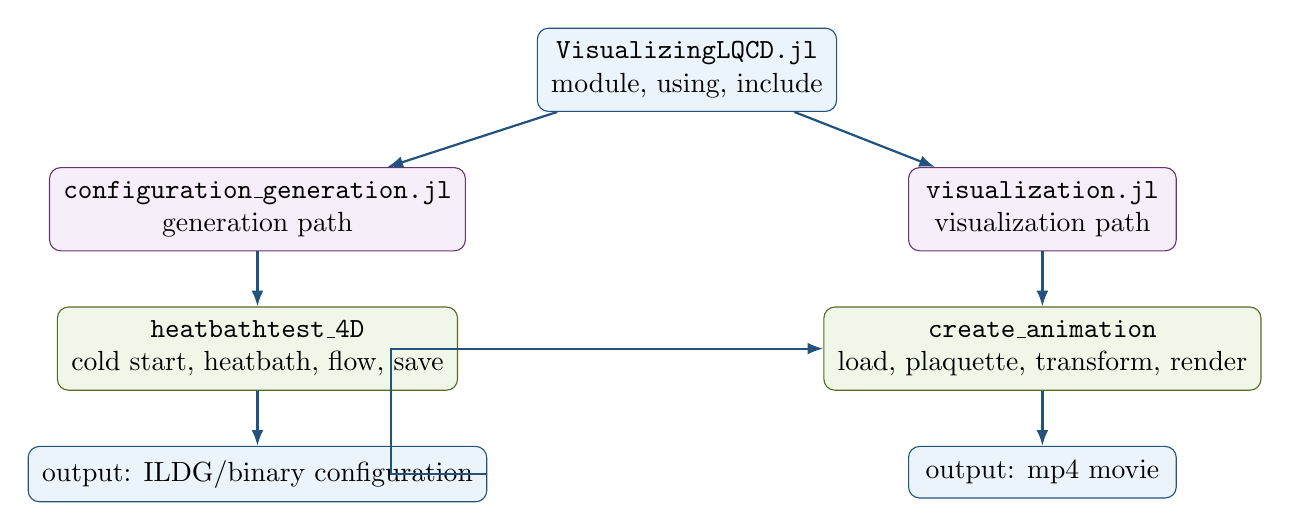
\begin{tikzpicture}[
  node distance=7mm and 9mm,
  box/.style={draw=accent, rounded corners, fill=lightaccent, inner sep=5pt, align=center, minimum width=34mm},
  pbox/.style={draw=accent2, rounded corners, fill=lightpurple, inner sep=5pt, align=center, minimum width=34mm},
  gbox/.style={draw=accent3, rounded corners, fill=lightgreen, inner sep=5pt, align=center, minimum width=34mm},
  arrow/.style={-{Latex[length=2mm]}, thick, color=accent}
]
\node[box] (module) {\code{VisualizingLQCD.jl}\\module, using, include};
\node[pbox, below left=of module] (genfile) {\code{configuration\_generation.jl}\\generation path};
\node[pbox, below right=of module] (visfile) {\code{visualization.jl}\\visualization path};
\node[gbox, below=of genfile] (genfunc) {\code{heatbathtest\_4D}\\cold start, heatbath, flow, save};
\node[gbox, below=of visfile] (visfunc) {\code{create\_animation}\\load, plaquette, transform, render};
\node[box, below=of genfunc] (conf) {output: ILDG/binary configuration};
\node[box, below=of visfunc] (movie) {output: mp4 movie};
\draw[arrow] (module) -- (genfile);
\draw[arrow] (module) -- (visfile);
\draw[arrow] (genfile) -- (genfunc);
\draw[arrow] (visfile) -- (visfunc);
\draw[arrow] (genfunc) -- (conf);
\draw[arrow] (conf) -- ++(1.7,0) |- (visfunc);
\draw[arrow] (visfunc) -- (movie);
\end{tikzpicture}
\caption{現行コードの大まかな実行時構造。生成 path と可視化 path は同じ module に入っているが、file 出力を介して接続される。}
\label{fig:current-code-flow}
\end{figure}

\subsection{全関数の入出力型一覧}
現行コードの多くの関数は、Julia の signature 上では型注釈を持たない。したがって、表では「宣言上の型」と「実際に期待される型」を分けて書く。宣言上の型がない引数は \code{Any} として受け取られるが、内部の配列確保、loop、Gaugefields API、Makie API により、実用上は \code{Int}、\code{Float64}、\code{String}、Gaugefields の field 型が期待される。戻り値についても、明示 \code{return} がない関数は side effect を主目的とし、戻り値に API 契約を置かない方が安全である。

{\footnotesize
\begin{longtable}{>{\raggedright\arraybackslash}p{0.20\linewidth}>{\raggedright\arraybackslash}p{0.31\linewidth}>{\raggedright\arraybackslash}p{0.21\linewidth}>{\raggedright\arraybackslash}p{0.21\linewidth}}
\caption{現行 source に定義される関数の I/O 型。}\label{tab:function-io}\\
\toprule
関数 & 入力 & 出力 & 副作用・注意点 \\
\midrule
\endfirsthead
\toprule
関数 & 入力 & 出力 & 副作用・注意点 \\
\midrule
\endhead
\code{automatic\_level2} & 宣言上は \code{plaqs\_t::Any}。実用上は \code{AbstractArray\{<:Real\}}。\code{minimum}, \code{maximum}, \code{mean}, \code{mode}, \code{std} が定義されている必要がある。 & \code{(level, isorange, min\_val, max\_val)}。実用上は実数 tuple。\code{level=mean(plaqs\_t)}、\code{isorange=std(plaqs\_t)}。 & 統計量を \code{println} で表示する。空配列や非数値配列では失敗する。level selection と診断表示が同じ関数に混ざっている。 \\
\code{ln\_a} & \code{beta} は厳密に \code{Float64}。 & \code{Float64}。\(\log(a/r_0)\) の fit 値。 & \(\beta\notin[5.7,6.57]\) で \code{ArgumentError} を投げる。\code{Int} や \code{Float32} には method がない。 \\
\code{calculate\_a} & \code{beta} は厳密に \code{Float64}。 & \code{Float64}。\(a=r_0\exp(\ln a)\) を fm 単位で返す。 & \code{ln\_a} に依存するため、同じ \(\beta\) 範囲制限を持つ。 \\
\code{create\_animation} & 宣言上は全 positional 引数と keyword が型なし。実用上は \code{NX, NY, NZ, NT, NC::Int}、\code{videoname::AbstractString}、\code{beta::Float64}、\code{filename::AbstractString}。 & 明示 return はない。最後の式は Makie の \code{record(...)} なので、戻り値は現在の Makie 実装に依存し、API 契約にしない方がよい。 & ILDG file を読み、mp4 などを \code{videoname} に書く。GLMakie figure を作る。\code{flow\_steps\_in} と \code{scale\_factor} は現行関数内では使われない。\code{levels[1]} が空 level に弱い。 \\
\code{heatbath\_SU3!} & 宣言上は全引数が型なし。実用上、\code{U} は4方向の Gaugefields gauge-link collection、\code{NC::Int}、\code{temps} は長さ5以上で \code{similar(U[1])} 型の作業 field 群、\code{β::Real}。 & \code{Nothing} と扱うのが自然。主出力は mutation された \code{U}。 & \code{U[μ]} を even/odd で破壊的に更新する。\code{temps[5]} を staple 作業領域として使う。\code{loops\_staple}、\code{SU3update\_matrix!}、\code{evaluate\_gaugelinks\_evenodd!}、\code{map\_U!} に依存する。 \\
\code{heatbathtest\_4D} & 宣言上は全引数が型なし。実用上は \code{NX, NY, NZ, NT, NC::Int}、\code{flow\_steps\_in::Int}、\code{β::Real}、\code{confname::AbstractString}。 & \code{plaq\_t}。実用上は最後に測った normalized plaquette の実数値。 & cold start から配位を生成し、heatbath 20 sweeps、gradient flow、\code{save\_binarydata(U, confname)} を実行する。標準出力に plaquette、Polyakov loop、progress を表示する。 \\
\code{test()} in \code{test/runtests.jl} & 入力なし。 & 明示 return はない。\code{create\_animation} の戻り値に依存しない smoke test と見るべきである。 & \(12^3\times16\) 配位を生成し、ILDG/binary file と mp4 を作る。GUI/backend と動画 encoder に依存するため通常 CI では重い。 \\
\bottomrule
\end{longtable}
}

\subsection{局所関数と匿名関数}
\code{heatbath\_SU3!} の内部には、\code{mapfunc!} という局所関数があり、この関数が \code{SU3update\_matrix!} を呼ぶ\cite{VisualizingConfig}。入力 \code{A} と \code{B} は Gaugefields の \code{map\_U!} から渡される link/staple 型の値であり、\code{mapfunc!} は \(\beta\)、\(N_c\)、作業行列、反復上限を closure として捕捉する。出力は \code{SU3update\_matrix!} の戻り値に依存するが、実質的な主出力は \code{A} の破壊的更新である。

\code{create\_animation} の内部には、\code{record(fig, videoname, 1:t\_end; framerate=framerate) do i ... end} の匿名関数がある\cite{VisualizingVisualization}。入力 \code{i} は frame index であり、現行コードでは \code{t = i \% NT + 1} によって第4方向 slice を選ぶ。出力値は使われず、主な副作用は既存 contour object の削除、新しい contour の描画、title 更新、動画 frame の記録である。ここは off-by-one を直す PR 0 の直接対象であり、\code{slice4=(i-1)\%NT+1} にすれば最初の frame が slice 1 になる。

\subsection{top-level 定数と実行時副作用}
\code{visualization.jl} は include 時に \code{GLMakie.activate!()} を実行し、さらに \code{LtoSec=10/3}、\code{myxlabel}、\code{myylabel}、\code{myzlabel}、\code{r\_0=0.48} を top-level 定数として定義する\cite{VisualizingVisualization}。このうち \code{LtoSec} は yoctosecond 表示を作るための値なので、時間表示廃止後は legacy default として隔離する。\code{r\_0} と \code{ln\_a} の多項式係数は物理単位換算に関わるため、\code{ScaleSpec} に移し、metadata に source と一緒に保存するのがよい。

\code{constants.jl} は、\code{NX=24}、\code{NY=24}、\code{NZ=24}、\code{NT=32}、\(\beta=6.0\)、\code{NC=3}、\code{flow\_steps\_in=200}、\code{confname}、\code{videoname} を top-level 変数として定義する\cite{VisualizingConstants}。現行 module からは使われていないため、PR では削除よりも \code{examples/} へ移す方が安全である。\code{header.jl} も同様に、module 本体が同じ依存を読むため、現行 package API には影響しない旧補助ファイルとして扱う\cite{VisualizingHeader}。

\subsection{I/O 型から見える改修方針}
この I/O 棚卸しから、最初に直すべき点は3つに絞れる。第一に、\code{create\_animation} の戻り値を曖昧な \code{record} 依存にせず、\code{AnimationResult} または \code{NamedTuple} として、\code{video\_path}、\code{metadata\_path}、\code{levels}、\code{raw\_equivalent\_levels} を返す。第二に、\code{heatbathtest\_4D} は \code{GenerationResult} を返し、\code{plaq\_t} だけでなく \code{confname}、\code{final\_plaquette}、\code{final\_polyakov}、\code{flow\_steps} を記録する。第三に、\code{automatic\_level2} は表示をやめ、\code{LevelStats} か named tuple を返す純粋関数へ変える。

型注釈は過剰に付ける必要はないが、API 境界では最低限の validation を入れるべきである。格子サイズは正の整数、\(N_c\) は正の整数、\(\beta\) は \code{Real} を受けて内部で \code{Float64} へ変換する、入力 file は存在確認する、出力 file の拡張子と backend は整合性を確認する。この validation を入れるだけで、現行の「深い依存関数の中で失敗する」挙動を減らせる。




\section{現行実装の詳細棚卸し}
\subsection{呼び出しグラフ}
現行コードで export される関数は \code{create\_animation} と \code{heatbathtest\_4D} である。非 export の helper は \code{automatic\_level2}、\code{ln\_a}、\code{calculate\_a}、\code{heatbath\_SU3!} であり、\code{test/runtests.jl} には package 外の \code{test()} が定義される\cite{VisualizingVisualization,VisualizingConfig,VisualizingTest}。呼び出し関係は小さいが、\code{create\_animation} の中に I/O、observable、transform、level、renderer が密結合している。したがって、関数数は少ないが、単体テスト可能な責務はかなり多い。

\begin{figure}[ht]
\centering
\resizebox{0.98\linewidth}{!}{%
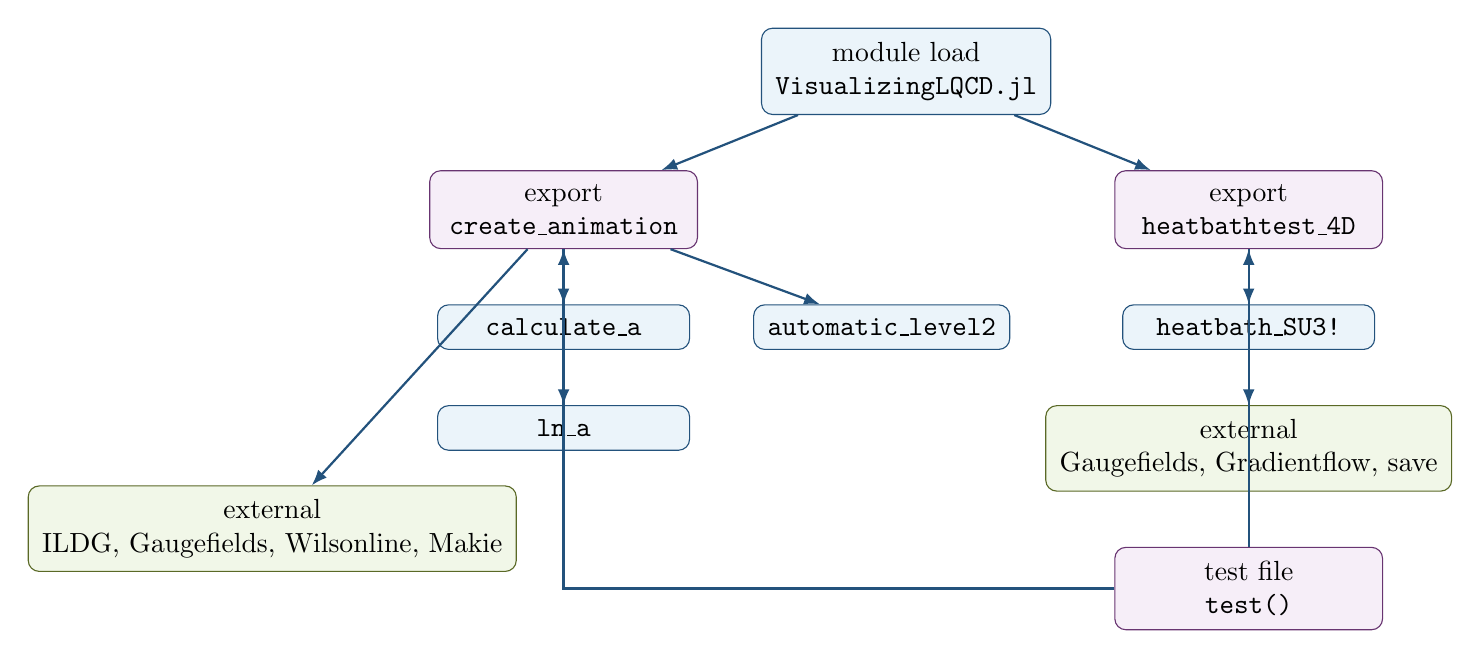
\begin{tikzpicture}[
  node distance=7mm and 8mm,
  box/.style={draw=accent, rounded corners, fill=lightaccent, inner sep=5pt, align=center, minimum width=32mm},
  ibox/.style={draw=accent2, rounded corners, fill=lightpurple, inner sep=5pt, align=center, minimum width=34mm},
  ebox/.style={draw=accent3, rounded corners, fill=lightgreen, inner sep=5pt, align=center, minimum width=36mm},
  arrow/.style={-{Latex[length=2mm]}, thick, color=accent}
]
\node[box] (module) {module load\\\code{VisualizingLQCD.jl}};
\node[ibox, below left=of module] (create) {export\\\code{create\_animation}};
\node[ibox, below right=of module] (generate) {export\\\code{heatbathtest\_4D}};
\node[box, below=of create] (calca) {\code{calculate\_a}};
\node[box, below=of calca] (lna) {\code{ln\_a}};
\node[box, right=of calca] (levels) {\code{automatic\_level2}};
\node[ebox, below=of create, xshift=-37mm, yshift=-23mm] (depvis) {external\\ILDG, Gaugefields, Wilsonline, Makie};
\node[box, below=of generate] (hb) {\code{heatbath\_SU3!}};
\node[ebox, below=of hb] (depgen) {external\\Gaugefields, Gradientflow, save};
\node[ibox, below=of depgen] (runtest) {test file\\\code{test()}};
\draw[arrow] (module) -- (create);
\draw[arrow] (module) -- (generate);
\draw[arrow] (create) -- (calca);
\draw[arrow] (calca) -- (lna);
\draw[arrow] (create) -- (levels);
\draw[arrow] (create) -- (depvis);
\draw[arrow] (generate) -- (hb);
\draw[arrow] (generate) -- (depgen);
\draw[arrow] (runtest) -- (generate);
\draw[arrow] (runtest) -| (create);
\end{tikzpicture}%
}
\caption{現行関数の呼び出しグラフ。関数数は少ないが、\code{create\_animation} が多数の責務を同時に担う。}
\label{fig:call-graph-current}
\end{figure}

\subsection{外部API依存の書き出し}
現行関数の型は、依存 package の API によって実質的に決まっている。\code{Initialize\_Gaugefields} はゲージ場の入れ物を作り、\code{ILDG} と \code{load\_gaugefield!} は file から配位を読み、\code{Wilsonline} と \code{evaluate\_gaugelinks!} はプラケット loop を評価する\cite{VisualizingVisualization}。\code{heatbathtest\_4D} 側では、\code{calculate\_Plaquette}、\code{calculate\_Polyakov\_loop}、\code{Gradientflow}、\code{flow!}、\code{save\_binarydata} が主要な外部 API である\cite{VisualizingConfig}。この依存表を作ると、切り出すべき境界が明確になる。

{\small
\begin{longtable}{p{0.20\linewidth}p{0.28\linewidth}p{0.22\linewidth}p{0.22\linewidth}}
\caption{現行コードが呼ぶ外部 API と分離先。}\label{tab:external-deps}\\
\toprule
外部 API & 現行での用途 & 依存元 & 分離後の置き場所 \\
\midrule
\endfirsthead
\toprule
外部 API & 現行での用途 & 依存元 & 分離後の置き場所 \\
\midrule
\endhead
\code{GLMakie.activate!()} & GLMakie backend を有効化する。 & top-level & \code{renderers.jl}。module include 時には実行しない。 \\
\code{Initialize\_}\newline\code{Gaugefields} & gauge field container を作る。 & \code{create\_animation}, \code{heatbathtest\_4D} & \code{io.jl} と \code{generation.jl}。 \\
\code{ILDG}, \code{load\_gaugefield!} & ILDG file を配位へ読む。 & \code{create\_animation} & \code{io.jl}。 \\
\code{Wilsonline} & plaquette path を Wilson line として表す。 & \code{create\_animation} & \code{observables.jl}。 \\
\code{Gaugefields.}\newline\code{evaluate\_gaugelinks!} & Wilson line に沿った link 積を全格子点で評価する。 & \code{create\_animation} & \code{observables.jl}。 \\
\code{tr}, \code{real} & SU(3) plaquette matrix から scalar を取る。 & \code{create\_animation} & \code{observables.jl}。 \\
\code{mean}, \code{std}, \code{mode} & 変換後 field の統計量を出す。 & \code{automatic\_level2} & \code{levels.jl} または \code{diagnostics.jl}。 \\
\code{Figure}, \code{Axis3}, \code{contour!}, \code{record} & 3D 等値面と動画を作る。 & \code{create\_animation} & \code{renderers.jl}。 \\
\code{loops\_staple} & heatbath staple loop の定義を得る。 & \code{heatbath\_SU3!} & \code{generation.jl}。 \\
\code{evaluate\_}\newline\code{gaugelinks\_evenodd!} & even/odd site の staple を評価する。 & \code{heatbath\_SU3!} & \code{generation.jl}。 \\
\code{SU3update\_}\newline\code{matrix!}, \code{map\_U!} & SU(3) link を破壊的に更新する。 & \code{heatbath\_SU3!} & \code{generation.jl}。 \\
\code{calculate\_}\newline\code{Plaquette} & 平均 plaquette を測る。 & \code{heatbathtest\_4D} & \code{generation.jl} または \code{measurements.jl}。 \\
\code{calculate\_}\newline\code{Polyakov\_loop} & Polyakov loop を測る。 & \code{heatbathtest\_4D} & \code{generation.jl} または \code{measurements.jl}。 \\
\code{Gradientflow}, \code{flow!} & gauge field を flow で滑らかにする。 & \code{heatbathtest\_4D} & \code{flow.jl}。 \\
\code{save\_binarydata} & 配位を file へ保存する。 & \code{heatbathtest\_4D} & \code{io.jl} または \code{generation.jl}。 \\
\bottomrule
\end{longtable}
}

\subsection{\texorpdfstring{\code{create\_animation}}{create_animation} の内部変数と形状}
\code{create\_animation} は、可視化 pipeline の全段階を1関数にまとめている。内部変数の多くは後続 PR で独立した型に移せる。とくに \code{U1}、\code{Uloop}、\code{temps} は Gaugefields/Wilsonloop 側の作業データであり、\code{plaqs\_t} は renderer へ渡すべき scalar field である。\code{levels}、\code{x\_physical}、tick label、\code{fig}、\code{ax}、\code{plot\_obj} は描画設定であり、observable の計算とは切り離せる。

{\small
\begin{longtable}{p{0.20\linewidth}p{0.24\linewidth}p{0.30\linewidth}p{0.18\linewidth}}
\caption{\code{create\_animation} の内部変数の棚卸し。}\label{tab:create-vars}\\
\toprule
変数 & 推定型・形状 & 意味 & 分離先 \\
\midrule
\endfirsthead
\toprule
変数 & 推定型・形状 & 意味 & 分離先 \\
\midrule
\endhead
\code{Nwing} & \code{Int}, 値0 & Gaugefields の wing 幅。 & \code{ConfigSpec}。 \\
\code{a} & \code{Float64} & \(\beta\) から推定した格子間隔 fm。 & \code{scales.jl}。 \\
\code{scale\_factor} & \code{Float64} & 現行では代入されるが未使用。 & 削除または \code{ScaleSpec}。 \\
\code{U1} & 4方向 gauge field collection & ILDG を読み込む入れ物。 & \code{io.jl}。 \\
\code{ildg} & ILDG reader object & 入力 file handle または reader。 & \code{io.jl}。 \\
\code{loop} & \code{Vector\{Tuple\{Int,Int\}\}} & \((1,+),(2,+),(1,-),(2,-)\) の plaquette path。 & \code{PlaquettePlane((1,2))}。 \\
\code{w} & Wilsonline object & \code{loop} を Wilsonloop.jl の表現へ変換したもの。 & \code{observables.jl}。 \\
\code{Uloop} & \code{similar(U1[1])} & 各点の plaquette matrix を保持する作業 field。 & \code{observables.jl}。 \\
\code{temps} & 長さ10の作業 field vector & Wilsonline 評価の temporary buffer。 & \code{observables.jl} 内部。 \\
\code{tmp} & \code{Float64} & \(1-\Re\tr U_{12}/N_c\) の raw plaquette deviation。 & \code{ScalarField.raw}。 \\
\code{plaqs\_t} & \code{Array\{Float64,4\}}, \((N_X,N_Y,N_Z,N_T)\) & \(-\log(tmp+10^{-7})\) 変換後 field。 & \code{ScalarField.display}。 \\
\code{level} & 実数 & 変換後 field の平均。 & \code{LevelStats}。 \\
\code{isorange} & 実数 & 変換後 field の標準偏差。 & \code{LevelStats}。 \\
\code{levels} & \code{Vector\{Float64\}} & 等値面の表示レベル。 & \code{LevelSpec} と \code{LevelResult}。 \\
\code{x\_physical} 等 & \code{Tuple\{Float64,Float64\}} & Makie contour に渡す座標範囲。 & \code{SpatialAxes}。 \\
\code{x\_positions} 等 & \code{StepRangeLen} & tick 位置。 & \code{AxisSpec}。 \\
\code{x\_labels} 等 & \code{Vector\{String\}} & tick label。1つおきに空文字へ変える。 & \code{AxisSpec}。 \\
\code{fig} & Makie \code{Figure} & 描画 canvas。 & \code{renderers.jl}。 \\
\code{ax} & Makie \code{Axis3} & 3D 軸。 & \code{renderers.jl}。 \\
\code{dummy\_data} & \code{Array\{Float64,3\}} & 最初の contour object を作るための空 field。 & renderer 内部。 \\
\code{plot\_obj} & Makie plot object & frame ごとに消して再作成される contour。 & renderer 内部。 \\
\code{framerate} & \code{Int}, 値12 & 動画 fps。 & \code{RenderSpec}。 \\
\code{t\_end} & \code{Int}, 現行 \code{NT*1} & frame 数。 & \code{FrameSpec}。 \\
\code{t} & \code{Int} & 第4方向 slice。現行は \code{i\%NT+1}。 & \code{frame\_map}。 \\
\code{t\_phys} & \code{Float64/String} & yoctosecond 表示用。廃止対象。 & legacy metadata。 \\
\bottomrule
\end{longtable}
}

\subsection{\texorpdfstring{\code{heatbath\_SU3!}}{heatbath_SU3!} と \texorpdfstring{\code{heatbathtest\_4D}}{heatbathtest_4D} の内部変数}
配位生成側は、可視化本体から外しても document には残すべきである。\code{heatbath\_SU3!} は破壊的更新関数であり、\code{heatbathtest\_4D} はデモ用 driver である。生成側の変数は、将来の \code{GenerationSpec}、\code{HeatbathSpec}、\code{FlowSpec}、\code{GenerationResult} に移せる。

{\small
\begin{longtable}{p{0.20\linewidth}p{0.24\linewidth}p{0.30\linewidth}p{0.18\linewidth}}
\caption{配位生成側の内部変数の棚卸し。}\label{tab:generation-vars}\\
\toprule
変数 & 推定型・形状 & 意味 & 分離先 \\
\midrule
\endfirsthead
\toprule
変数 & 推定型・形状 & 意味 & 分離先 \\
\midrule
\endhead
\code{Dim} & \code{Int}, 値4 & 4次元 Euclidean 格子。 & \code{LatticeSpec}。 \\
\code{V} & Gaugefields field & \code{temps[5]} を staple 作業領域として使用。 & \code{HeatbathWorkspace}。 \\
\code{ITERATION\_MAX} & \code{Int}, 値100000 & \code{SU3update\_matrix!} の反復上限。 & \code{HeatbathSpec}。 \\
\code{temps2} & 長さ5の \(2\times2\) complex matrix vector & SU(2) subgroup 更新用の作業行列と推定される。 & \code{HeatbathWorkspace}。 \\
\code{temps3} & 長さ5の \(N_c\times N_c\) complex matrix vector & SU(3) 更新用の作業行列。 & \code{HeatbathWorkspace}。 \\
\code{mapfunc!} & 局所関数 & \(A,B\) を受けて \code{SU3update\_matrix!} を呼ぶ closure。 & \code{heatbath\_kernel!}。 \\
\code{loops} & Gaugefields loop object & \code{loops\_staple[(Dim,mu)]} から得る staple path。 & \code{HeatbathSpec}。 \\
\code{iseven} & \code{Bool} & even/odd site の切替。 & update loop 内部。 \\
\code{U} & 4方向 gauge field collection & cold start で作った生成対象。 & \code{GenerationState}。 \\
\code{temp1}--\code{temp5} & \code{similar(U[1])} & plaquette、Polyakov、heatbath の作業 field。 & \code{GenerationWorkspace}。 \\
\code{comb} & \code{Int}, 値6 & 4次元の面数 \(\binom{4}{2}\)。 & \code{binomial(Dim,2)}。 \\
\code{factor} & 実数 & plaquette 正規化係数 \(1/(6\,NV\,N_c)\)。 & \code{PlaquetteNormalization}。 \\
\code{plaq\_t} & 実数 & 正規化 plaquette。戻り値。 & \code{GenerationResult}。 \\
\code{poly} & 複素数 & Polyakov loop。現行では表示だけ。 & \code{GenerationResult}。 \\
\code{numhb} & \code{Int}, 値20 & heatbath sweep 数。 & \code{HeatbathSpec}。 \\
\code{g} & Gradient flow object & \code{Gradientflow(U)} の戻り値。 & \code{FlowState}。 \\
\code{flow\_steps} & \code{Int} & gradient flow の繰り返し回数。 & \code{FlowSpec}。 \\
\code{filename} & \code{String} & \code{confname} を代入した保存先。 & \code{GenerationResult}。 \\
\bottomrule
\end{longtable}
}

\subsection{関数ごとの失敗条件と validation}
現行コードは、多くの前提を深い依存関数に任せている。利用者向け API にするなら、入口で検査した方が原因が分かりやすい。たとえば \(\beta\) の範囲外は \code{ln\_a} が \code{ArgumentError} を投げるが、file が存在しない場合、ILDG の格子サイズと引数が合わない場合、level 列が空の場合、GLMakie backend が使えない場合は、より上流で明示した方がよい。

{\small
\begin{longtable}{p{0.22\linewidth}p{0.34\linewidth}p{0.34\linewidth}}
\caption{現行関数の主な失敗条件と追加すべき validation。}\label{tab:failure-modes}\\
\toprule
対象 & 起こり得る失敗 & 追加すべき検査・対策 \\
\midrule
\endfirsthead
\toprule
対象 & 起こり得る失敗 & 追加すべき検査・対策 \\
\midrule
\endhead
\code{automatic\_level2} & 空配列、NaN だけの配列、\code{mode} が重いまたは非数値。 & finite 値だけを抽出し、空なら明示 error。\code{mode} は任意診断へ移す。 \\
\code{ln\_a} & \code{Float64} 以外に method がない。範囲外で error。 & \code{Real} を受けて内部で \code{Float64} 化。範囲外では lattice units fallback を選べるようにする。 \\
\code{calculate\_a} & \code{ln\_a} と同じ。 & \code{ScaleSpec} に source、範囲、fallback を持たせる。 \\
\code{create\_animation} & 入力 file がない。file 中の格子サイズと引数が違う。\(N_c\) が違う。 & file 存在確認、lattice shape 照合、\(N_c\) 照合、読み込み後の sanity check。 \\
\code{create\_animation} & \code{levels} が空になり、\code{levels[1]} で失敗。 & level selection が空なら fallback level を作るか、明示 error を出す。 \\
\code{create\_animation} & \code{tmp<0} や丸め誤差で \code{-log(tmp+eps)} が問題化する。 & raw を \code{max(tmp,0)} で扱うか、負値 count を metadata に保存する。 \\
\code{create\_animation} & GLMakie/encoder が headless 環境で失敗。 & backend を \code{:auto} にし、CI は CairoMakie 静止画 smoke test にする。 \\
\code{create\_animation} & 最初の frame が slice 2 になる。 & \code{slice4=(i-1)\%NT+1} へ変更し、unit test を追加。 \\
\code{heatbath\_SU3!} & \code{temps} が短い、\code{temps[5]} が合わない、\(N_c\ne3\) で SU3 専用関数と齟齬。 & \code{length(temps)>=5}、field shape、\(N_c=3\) または実対応範囲を入口で明示。 \\
\code{heatbathtest\_4D} & 格子サイズが非正、flow step が負、保存先 directory がない。 & \code{GenerationSpec} で validate。保存先 directory を確認。 \\
\code{test()} & 動画生成が CI で重い、backend 依存で不安定。 & 通常 test と heavy integration test を分ける。 \\
\bottomrule
\end{longtable}
}

\subsection{現行処理を段階名へ写した疑似コード}
以下の疑似コードは、現行 \code{create\_animation} の処理を段階名に置き換えたものである。現行の動作を保ったまま、分割後の関数名を与えるとこうなる。PR では、この順序を変えずに関数を分けると、回帰確認が容易になる。

\begin{lstlisting}[style=julia,caption={現行 create-animation を段階化した疑似コード}]
function current_create_animation_pipeline(args)
    # 1. Scale
    a = calculate_a(beta)

    # 2. I/O
    U = allocate_gaugefield(NC, Nwing, NX, NY, NZ, NT)
    load_configuration!(U, filename; lattice=(NX,NY,NZ,NT), nc=NC)

    # 3. Observable
    Uloop = evaluate_wilsonline(U, loop=[(1,+1),(2,+1),(1,-1),(2,-1)])
    raw = Array{Float64}(undef, NX, NY, NZ, NT)
    for x,y,z,t in lattice_sites
        raw[x,y,z,t] = 1 - real(tr(Uloop[:,:,x,y,z,t])) / NC
    end

    # 4. Display transform, current-compatible
    display = -log.(raw .+ 1e-7)

    # 5. Level selection, current-compatible
    level = mean(display)
    isorange = std(display)
    levels = collect((level + 1.2 * isorange):0.05:maximum(display))

    # 6. Rendering
    axes = physical_axes(a, NX, NY, NZ)
    frame_map = [(frame=i, slice4=(i % NT) + 1) for i in 1:NT]
    render_makie_movie(display, axes, levels, frame_map, videoname)
end
\end{lstlisting}

\subsection{推奨する戻り値契約}
現行 \code{create\_animation} は、動画 file を書く副作用を主目的にし、戻り値を明示しない。改善版では、処理結果を返す。戻り値があれば、動画を開かなくてもテストで level、frame map、metadata path を確認できる。配位生成側も同様に、最後の plaquette だけでなく、保存 file、flow step、Polyakov loop、測定履歴を返す。

\begin{lstlisting}[style=julia,caption={戻り値契約の型案}]
struct AnimationResult
    video_path::String
    metadata_path::String
    lattice::NTuple{4,Int}
    nc::Int
    beta::Union{Nothing,Float64}
    observable_name::String
    transform_name::String
    epsilon::Float64
    display_levels::Vector{Float64}
    raw_equivalent_levels::Vector{Float64}
    frame_map::Vector{NamedTuple}
end

struct GenerationResult
    configuration_path::String
    lattice::NTuple{4,Int}
    nc::Int
    beta::Float64
    heatbath_sweeps::Int
    flow_steps::Int
    final_plaquette::Float64
    final_polyakov::ComplexF64
end
\end{lstlisting}

\subsection{推奨する関数シグネチャ一覧}
型を付けすぎると Julia の柔軟性を損なうため、内部関数は抽象型で受けてよい。ただし、public API と file 境界は明示する。以下は、v7 で提案する最小限の書き換え先である。

{\small
\begin{longtable}{p{0.28\linewidth}p{0.62\linewidth}}
\caption{現行関数から移行する推奨シグネチャ。}\label{tab:proposed-signatures}\\
\toprule
責務 & 推奨シグネチャ \\
\midrule
\endfirsthead
\toprule
責務 & 推奨シグネチャ \\
\midrule
\endhead
設定 validation & \code{validate(spec::ConfigSpec)::Nothing} \\
格子間隔 & \code{lattice\_spacing\_fm(beta::Real, scale::ScaleSpec)::Float64} \\
配位読み込み & \code{load\_configuration(spec::ConfigSpec)::Any} \\
frame map & \code{make\_frame\_map(NT::Integer; loops::Integer=1)::Vector\{NamedTuple\}} \\
単一面 plaquette & \code{measure(U, obs::PlaquettePlane)::ScalarField} \\
全 plaquette 和 & \code{measure(U, obs::PlaquetteSum)::ScalarField} \\
表示変換 & \code{build\_display\_field(raw::ScalarField, spec::TransformSpec)::FieldBundle} \\
level 選択 & \code{choose\_levels(data::AbstractArray, spec::LevelSpec)::LevelResult} \\
逆変換 & \code{invert\_display\_levels(levels, spec::TransformSpec, epsilon::Real)::Vector\{Float64\}} \\
描画 & \code{render\_movie(field::ScalarField, axes::SpatialAxes, levels::Vector, frames, spec::RenderSpec)::String} \\
metadata & \code{write\_metadata(path::AbstractString, result::AnimationResult)::String} \\
統合 API & \code{visualize\_lqcd(spec::ConfigSpec; kwargs...)::AnimationResult} \\
互換 wrapper & \code{create\_animation(...; kwargs...)::AnimationResult} \\
heatbath 更新 & \code{heatbath\_SU3!(U, spec::HeatbathSpec, workspace)::Nothing} \\
配位生成 & \code{generate\_quenched(spec::GenerationSpec)::GenerationResult} \\
\bottomrule
\end{longtable}
}

\subsection{metadata に現行値から書き出せる項目}
現行コードだけからでも、かなり多くの情報を metadata に書ける。重要なのは、動画の見た目を決めた値と、物理的解釈に必要な値を同時に残すことである。たとえば \code{loop}、\code{epsilon}、\code{levels}、\code{beta}、\code{a}、\code{r\_0}、\code{framerate}、\code{figure size}、\code{colormap}、\code{frame map} はすべて現行関数内で分かる。したがって、metadata 追加は大きな構造変更なしでも PR 2 より前に入れられる。

\begin{lstlisting}[style=json,caption={現行 create-animation から直接書き出せる metadata 項目}]
{
  "lattice": [NX, NY, NZ, NT],
  "nc": NC,
  "beta": beta,
  "lattice_spacing_fm": a,
  "scale": {"r0_fm": 0.48, "beta_range": [5.7, 6.57]},
  "input_file": filename,
  "output_video": videoname,
  "observable": {
    "kind": "PlaquettePlane",
    "plane": [1, 2],
    "loop": [[1, 1], [2, 1], [1, -1], [2, -1]],
    "raw_formula": "1 - real(tr(Uloop))/NC"
  },
  "transform": {
    "kind": "neglog",
    "epsilon": 1e-7,
    "formula": "-log(raw + epsilon)",
    "raw_focus_for_upper_levels": "low_raw_deviation"
  },
  "levels": {
    "method": "mean_std_legacy",
    "mean": level,
    "std": isorange,
    "start": level + 1.2 * isorange,
    "step": 0.05,
    "display_values": levels,
    "raw_equivalent_values": [exp(-L) - 1e-7 for L in levels]
  },
  "render": {
    "backend": "GLMakie",
    "figure_size": [800, 800],
    "colormap": "viridis",
    "alpha": 1.0,
    "framerate": 12,
    "screen_time_label": false
  },
  "frame_map": [{"frame": i, "slice4": ((i - 1) % NT) + 1}]
}
\end{lstlisting}

\subsection{最小修正で追加できる実装片}
完全な分割を待たず、現行 \code{create\_animation} に小さな関数を足すだけでも改善できる。以下の関数は Gaugefields に依存しないため、すぐに単体テストできる。最初にこれを入れると、時間表示廃止、frame order 修正、対数 level の解釈保存が同時に進む。

\begin{lstlisting}[style=julia,caption={現行コードへ先に足せる純粋関数}]
make_frame_map(NT::Integer; loops::Integer=1) = [
    (frame=i, slice4=((i - 1) % NT) + 1) for i in 1:(NT * loops)
]

raw_equivalent_level_neglog(L::Real; epsilon::Real=1e-7) =
    max(exp(-Float64(L)) - Float64(epsilon), 0.0)

function legacy_mean_std_levels(display::AbstractArray; multiplier=1.2, step=0.05)
    values = collect(skipmissing(vec(display)))
    filter!(isfinite, values)
    isempty(values) && error("no finite display values")
    mu, sigma = mean(values), std(values)
    start = mu + multiplier * sigma
    stop = maximum(values)
    start > stop && return [stop]
    return collect(start:step:stop)
end
\end{lstlisting}


\section{現行コードのマジックナンバーを参考値として残す}
\subsection{基本方針}
現行コードに含まれる固定値は、単に消すのではなく、移行時の比較基準として記録する。とくに \(\epsilon=10^{-7}\)、\(\mu+1.2\sigma\) から始める等値面レベル、level 刻み \(0.05\)、framerate \(12\) は、既存動画の見え方を再現するために重要である\cite{VisualizingVisualization}。v7 では、これらを「legacy default」または「reference value」として metadata と設定型に移し、意味が曖昧なハードコードを減らす。値そのものをすべて推奨値とみなすのではなく、互換 wrapper、回帰テスト、発表済み動画との比較に使う。

\subsection{可視化経路の参考値}
\begin{description}[style=nextline,leftmargin=7em,labelwidth=6em]
  \item[\(10^{-7}\)] \code{-log(tmp + 0.0000001)} の \(\epsilon\) である。ゼロ近傍を避け、対数変換後の閾値選択を安定化するため、\code{TransformSpec(:neglog, 1e-7, :fixed, ...)} の legacy default として残す。
  \item[\(1.2\sigma\) と \(0.05\)] 現行コードは \code{mean + 1.2*std} から始め、\code{0.05} 刻みで \code{max} まで level を作る。新既定は分位点方式にするが、旧方式は \code{LevelSpec(:mean\_std)} として残し、raw equivalent value と一緒に metadata へ保存する。
  \item[\code{automatic\_level2}] \code{mean}, \code{mode}, \code{std}, \code{min}, \code{max} を表示する診断関数である。今後は histogram、分位点、voxel count、level 感度と合わせて metadata に残す。
  \item[\code{:neglog}] 現行の \code{-log(tmp + eps)} は、上側 level が raw \(p\) の小さい側を強調する。既存互換の表示変換として名前を付け、metadata に \code{raw\_focus="low\_raw\_deviation"} を保存する。
  \item[\code{xy} plaquette] Wilsonline は \code{[(1,+1),(2,+1),(1,-1),(2,-1)]} で、\(xy\) 面の \(1\times1\) プラケットを表す。この値は \code{PlaquettePlane((1,2))} として observable 名へ移す。
  \item[作業配列 10個] \code{temps = [similar(U1[1]) for \_ in 1:10]} は Wilsonline 評価の作業領域である。必要数を関数化し、observable 実装の内部詳細として隠す。
  \item[\code{beta=6.1}] \code{create\_animation} の default であり、README 例の \(\beta=6.0\) とは異なる。新 API では \(\beta\) を明示入力にし、この値は互換 wrapper にだけ残す。
  \item[既定ファイル名] \code{filename="conf\_00000100.ildg"} は現行 default である。新 API では入力ファイルを必須引数にし、互換 wrapper の fallback としてだけ残す。
  \item[\code{flow\_steps\_in=200}] \code{create\_animation} の default だが、現行関数内では使われない。README の scratch 生成例では 200 steps を使うため、\code{FlowSpec.steps} へ移し、読み込み後に flow を行うかどうかを明示する。
\end{description}

\subsection{描画と画面構成の参考値}
\begin{description}[style=nextline,leftmargin=7em,labelwidth=6em]
  \item[\code{LtoSec=10/3}] fm/\(c\) を yoctosecond へ換算する表示用値である。時間表示を止める方針により、画面からは廃止する。旧動画の再現に必要な場合だけ legacy metadata に残す。
  \item[\(800\times800\)] \code{Figure(size=(800,800))} の canvas サイズである。\code{RenderSpec} に移す。
  \item[色と透明度] \code{colormap=:viridis}, \code{transparency=false}, \code{alpha=1.0} は現行の描画 style である。\code{RenderStyle} に移し、metadata に保存する。
  \item[軸設定] \code{aspect=(1,1,1)}、tick label の \code{digits=2}、tick label を1つおきに消す stride \(2\) は見た目の設定である。\code{AxisSpec} として名前を付ける。
  \item[動画設定] \code{framerate=12} と \code{t\_end=NT*1} は、12 fps で第4方向を1周だけ再生する指定である。\code{RenderSpec} と \code{FrameSpec} に移す。
  \item[フレーム順序] 現行の \code{t = i \% NT + 1} は最初の frame が slice 2 になる。\code{slice4=(i-1)\%NT+1} に直し、frame map を JSON sidecar に保存する。
  \item[時刻整形] \code{round(t\_phys,digits=3)} と \code{lpad(...,6,'0')} は yoctosecond 表示のための整形である。時間表示の廃止に伴い legacy 扱いにする。
\end{description}

\subsection{スケール設定と配位生成の参考値}
\begin{description}[style=nextline,leftmargin=7em,labelwidth=6em]
  \item[\(r_0=0.48\,\mathrm{fm}\)] 現行の物理単位換算で使う Sommer scale である。\code{ScaleSpec(:r0,0.48)} として source と一緒に metadata に保存する。
  \item[\(\beta\) 範囲] \code{ln\_a(beta)} の適用範囲は \([5.7,6.57]\) である。範囲外では error にするか、lattice units 表示へ fallback するかを \code{ScaleSpec} で選ぶ。
  \item[3次多項式係数] \code{ln\_a(beta)} は \(-1.6805,-1.7139,0.8155,-0.6667\) を使う。係数は \code{ScaleSpec} に閉じ込め、source とともに metadata へ保存する。
  \item[\code{Dim=4}, \code{Nwing=0}] 4次元 Euclidean 格子と halo/wing 幅の設定である。\code{Dim} は \code{ConfigSpec.lattice} から導き、\code{Nwing} は I/O と generation の設定に残す。
  \item[初期条件] \code{condition="cold"} は配位生成デモの cold start を表す。\code{GenerationSpec} に移す。
  \item[更新上限] \code{ITERATION\_MAX=100000} は SU(3) 更新の反復上限である。\code{HeatbathSpec} にする。
  \item[作業配列 5個] \code{temps2} と \code{temps3} の長さ 5 は heatbath 更新の実装詳細である。更新アルゴリズム内へ閉じ込める。
  \item[\code{comb=6}] 4次元での \(\mu<\nu\) 面数である。固定値ではなく \code{binomial(Dim,2)} から計算する。
  \item[heatbath 20 sweeps] \code{numhb=20} はデモ用の sweep 数である。\code{GenerationSpec} として名前を付ける。
  \item[表示間隔 5 sweeps] \code{itrj \% 5 == 0} は plaquette と Polyakov loop の表示間隔である。\code{GenerationSpec} に移す。
  \item[flow step size 0.01] コメントに \code{flow\_time*0.01} とあり、flow step size が 0.01 であることを示唆している。\code{FlowSpec} として明示する。
\end{description}

\subsection{README と test の参考値}
README の例は、\(24^3\times32\)、\(\beta=6.0\)、\(N_c=3\)、scratch 生成では \code{flow\_steps\_in=200} を使う\cite{VisualizingReadme}。test は \(12^3\times16\)、\(\beta=6.0\)、\(N_c=3\)、\code{flow\_steps\_in=10} を使い、配位生成と動画生成をまとめて走らせる\cite{VisualizingTest}。これらは production default ではなく、demo size と CI smoke size として名前を付ける。たとえば \code{ExampleSpec(:readme)} と \code{ExampleSpec(:ci\_small)} を分けると、README、テスト、回帰比較の意図が混ざらない。

\begin{lstlisting}[style=julia,caption={同梱 skeleton に入れた reference default の例}]
const CURRENT_LOG_EPSILON = 1e-7
const CURRENT_LEVEL_STD_MULTIPLIER = 1.2
const CURRENT_LEVEL_STEP = 0.05
const CURRENT_MOVIE_FRAMERATE = 12
const CURRENT_MOVIE_NLOOPS = 1
const CURRENT_FIGURE_SIZE = (800, 800)
const CURRENT_COLORMAP = :viridis
const CURRENT_ALPHA = 1.0
const CURRENT_BETA_ANIMATION_DEFAULT = 6.1
const CURRENT_R0_FM = 0.48
const CURRENT_BETA_RANGE = (5.7, 6.57)
const CURRENT_LN_A_COEFFS = (-1.6805, -1.7139, 0.8155, -0.6667)
const CURRENT_HEATBATH_SWEEPS = 20
const CURRENT_HEATBATH_REPORT_INTERVAL = 5
const CURRENT_FLOW_STEP_SIZE = 0.01
\end{lstlisting}

\begin{proposalbox}{v7 の追加提案}
現行コードの固定値は、\code{current\_defaults.jl} と metadata schema にまとめる。旧動画を再現したい場合は \code{LegacyVisualDefaults()} を選び、研究用の新規動画では \code{QuantileLogDefaults()} などを選ぶ。値を明文化すれば、どの値が物理 convention で、どの値が表示 style で、どの値が単なる demo size かを利用者が判断できる。
\end{proposalbox}

\section{時間表示を止める}
\subsection{物理的な理由}
動画のフレームは第4方向スライスの走査であり、実時間の運動ではない。README の real time という表現と、コード中の yoctosecond タイトルは、見た目の説明としては直感的だが、発表や教材では誤解を生みやすい\cite{VisualizingReadme,VisualizingVisualization}。したがって、画面には時間を出さない。フレーム番号と第4方向スライスの対応は metadata に保存し、動画の見た目からは実時間の印象を取り除く。

この変更は情報を捨てるものではない。frame map を JSON sidecar に残せば、動画の第 \(i\) フレームがどの lattice slice に対応するかは復元できる。再現性は metadata が担い、画面表示は物理的に誤読されにくい表現にする。

\begin{lstlisting}[style=julia,caption={時間表示を削る最小修正の骨子}]
# Remove LtoSec and yoctosecond conversion from the display path.
static_title = "Plaquette log iso-surface"
record(fig, videoname, 1:t_end; framerate=movie_framerate) do i
    slice4 = (i - 1) % NT + 1
    delete!(ax, plot_obj)
    field3 = @view field4[:, :, :, slice4]
    # Keep the title static. No time or slice label is shown by default.
    ax.title = static_title
    plot_obj = GLMakie.contour!(ax, x_physical, y_physical, z_physical, field3;
                                levels=levels, colormap=:viridis,
                                transparency=false, alpha=1.0)
end
\end{lstlisting}

\subsection{表示と metadata の分担}
画面仕様は単純にする。既定タイトルは、\code{Plaquette log iso-surface} のように observable と transform だけを示す。フレーム番号、第4方向スライス、flow step、\(\beta\)、格子サイズ、\(\epsilon\)、level は、動画ではなく JSON sidecar に保存する。必要な利用者には \code{show\_frame\_label=true} を用意してよいが、既定値は \code{false} にする。

\section{対数変換を閾値座標として設計する}
\subsection{raw 量と表示変換を分ける}
プラケット deviation
\begin{equation}
  p(x)=1-\frac{1}{\Nc}\Ree\tr U_{\mu\nu}(x)
\end{equation}
は、格子間隔が小さい極限で \(F_{\mu\nu}^2\) 型の局所量に対応する非負スカラーである。Wilson の格子ゲージ理論は、リンク変数のゲージ不変な閉路積から作用を構成する標準的な枠組みを与える\cite{Wilson1974}。しかし、等値面描画で raw \(p\) をそのまま閾値座標に使う必要はない。可視化では、\(p\) から単調変換 \(f(p)\) を作り、その \(f\) 空間で等値面レベルを決める方が安定な場合がある。

対数は、乗法的な変化を加法的な変化へ写す。たとえば raw 値が2倍変わると、\(\log p\) は \(\log 2\) だけ変わる。これは、plaquette deviation の分布が細い本体と長い尾を持つとき、または gradient flow の step 数で値域が大きく変わるときに役立つ。したがって、対数は「物理量の定義」ではなく「閾値を置く座標系」である。

\begin{logbox}{v7 の解釈}
\(-\log(p+\epsilon)\) は、等値面の閾値選択を安定化する display transform である。raw 物理量 \(p\) は保持し、変換後の \(f(p)\) でレベルを選び、選んだレベルを raw \(p\) の閾値へ逆変換して metadata に保存する。この分離により、見やすさと物理的な説明を両立できる。
\end{logbox}

\subsection{符号の向きを仕様に入れる}
\(\ell_+(x)=\log(p(x)+\epsilon)\) は、\(p\) が大きいほど大きい。上側分位点で等値面を取ると、raw plaquette deviation の大きい領域が強調される。一方、\(\ell_-(x)=-\log(p(x)+\epsilon)\) は、\(p\) が小さいほど大きい。上側分位点で等値面を取ると、raw plaquette deviation の小さい領域が強調される。

この違いを曖昧にすると、動画の解釈を誤る。v7 では、transform に \code{:log} と \code{:neglog} を用意し、metadata に \code{raw\_focus} を記録する。既存動画の見え方を保つ場合は \code{:neglog} を既定にできるが、その時は \code{raw\_focus="low\_raw\_deviation"} と明示する。強い plaquette deviation の hot spot を見せたい場合は \code{:log} または \code{:identity} を選ぶ。

\begin{longtable}{p{0.18\linewidth}p{0.25\linewidth}p{0.23\linewidth}p{0.24\linewidth}}
\toprule
変換 & 表示値 & 上側レベルの意味 & 推奨説明 \\
\midrule
\code{:identity} & \(p\) & raw \(p\) が大きい領域 & plaquette deviation iso-surface \\
\code{:log} & \(\log(p+\epsilon)\) & raw \(p\) が大きい領域 & log plaquette-deviation iso-surface \\
\code{:neglog} & \(-\log(p+\epsilon)\) & raw \(p\) が小さい領域 & negative-log plaquette-deviation iso-surface \\
\bottomrule
\end{longtable}

\subsection{\texorpdfstring{$\epsilon$}{epsilon} を隠さない}
現状の \(10^{-7}\) は、ゼロや極小値に対する数値的な保護として使われている\cite{VisualizingVisualization}。ただし、\(p\) が \(\epsilon\) に近い領域では、\(\log(p+\epsilon)\) の値が \(\epsilon\) に敏感になる。したがって、\(\epsilon\) はハードコードされた内部定数ではなく、\code{TransformSpec} の明示フィールドにする。

互換性を重視するなら既定値は \(10^{-7}\) にする。研究発表用には、固定値を使うか、正の \(p\) の低分位点から自動決定する。自動決定を使う場合も、最終的に採用した \(\epsilon\) を metadata に保存する。

\begin{lstlisting}[style=julia,caption={対数変換を明示する型案}]
abstract type AbstractTransform end

struct TransformSpec <: AbstractTransform
    kind::Symbol              # :identity, :log, :neglog, :zscore
    epsilon::Float64          # default 1e-7 for current compatibility
    epsilon_policy::Symbol    # :fixed or :auto_quantile
    clip_quantiles::Tuple{Float64,Float64}
end

function display_transform(raw::AbstractArray, spec::TransformSpec)
    p = clamp.(raw, 0.0, Inf)
    eps = choose_epsilon(p, spec)
    if spec.kind == :identity
        return p, eps, "raw"
    elseif spec.kind == :log
        return log.(p .+ eps), eps, "log(raw + epsilon)"
    elseif spec.kind == :neglog
        return .-log.(p .+ eps), eps, "-log(raw + epsilon)"
    else
        error("unknown transform kind: $(spec.kind)")
    end
end
\end{lstlisting}

\subsection{level の逆変換を必ず残す}
変換後レベル \(L\) は raw \(p\) へ戻せる。\(\ell_+=\log(p+\epsilon)\) なら、
\begin{equation}
  p_{\mathrm{level}}=\exp(L)-\epsilon
\end{equation}
である。\(\ell_-=-\log(p+\epsilon)\) なら、
\begin{equation}
  p_{\mathrm{level}}=\exp(-L)-\epsilon
\end{equation}
である。これを保存すれば、動画で使った等値面が raw plaquette deviation のどの閾値に対応したかを後から確認できる。

\begin{lstlisting}[style=julia,caption={レベル逆変換の純粋関数案}]
function invert_display_level(level::Real, spec::TransformSpec, epsilon::Real)
    if spec.kind == :identity
        return Float64(level)
    elseif spec.kind == :log
        return max(exp(level) - epsilon, 0.0)
    elseif spec.kind == :neglog
        return max(exp(-level) - epsilon, 0.0)
    else
        error("level inversion is not defined for $(spec.kind)")
    end
end
\end{lstlisting}

\section{閾値選択を安定化する}
\subsection{分位点を既定にする}
現状コードは、変換後データの平均と標準偏差からレベル列を作る\cite{VisualizingVisualization}。この方法は簡単だが、外れ値、非対称分布、flow step の違いに敏感である。既定は分位点にする。たとえば \(q=0.80,0.90,0.95,0.98\) を使えば、「変換後値の上位20\%、10\%、5\%、2\%付近の面」という意味が残る。

分位点は、可視化の比較にも向いている。格子サイズや \(\beta\)、flow step、observable が変わっても、面の体積分率に近い意味を保てる。絶対値レベルが必要な場合は \code{:fixed} を選び、raw equivalent value を併記する。

\begin{lstlisting}[style=julia,caption={level selection の型案}]
struct LevelSpec
    method::Symbol            # :quantile, :fixed, :mean_std, :target_fraction
    quantiles::Vector{Float64}
    values::Vector{Float64}
    tail::Symbol              # :upper, :lower, :explicit
    global_across_slices::Bool
end

function choose_levels(display_data, spec::LevelSpec)
    values = collect(vec(display_data))
    filter!(isfinite, values)
    isempty(values) && error("display field has no finite values")

    if spec.method == :quantile
        return unique(sort(quantile(values, spec.quantiles)))
    elseif spec.method == :fixed
        return unique(sort(spec.values))
    elseif spec.method == :mean_std
        mu, sigma = mean(values), std(values)
        sigma == 0 && return [mu]
        return collect((mu + 1.2sigma):0.05:maximum(values))
    else
        error("unknown level-selection method: $(spec.method)")
    end
end
\end{lstlisting}

\subsection{global level を既定にする}
動画の各フレームで別々に分位点を計算すると、等値面の量が一定に見えやすいが、フレーム間の絶対的な強弱が消える。現状コードは4次元配列全体からレベルを決めるので、この点では global level になっている\cite{VisualizingVisualization}。v7 でも既定は \code{global\_across\_slices=true} とする。

一方で、教材やデモでは各フレームの構造を見せたい場合がある。その場合は local level を選べるようにする。ただし、metadata に \code{global\_across\_slices=false} と明記し、フレームごとの level 値を保存する。これにより、動画の比較可能性を後から判断できる。

\subsection{閾値感度を診断する}
閾値に敏感な可視化では、レベルを少し変えるだけで等値面が大きく変わる。そこで、各 level \(L\) について、\(V(L)=|\{x:f(x)\ge L\}|\) を保存する。さらに、\(L\pm\Delta L\) での変化率
\begin{equation}
  S(L)=\frac{|V(L+\Delta L)-V(L-\Delta L)|}{V(L)+1}
\end{equation}
を記録する。\(S(L)\) が大きい level は、見た目が閾値に強く依存している。

\begin{proposalbox}{閾値安定性の実装方針}
動画生成時に、raw と display の histogram、分位点、level ごとの voxel count、level 感度 \(S(L)\) を JSON sidecar に保存する。これにより、対数変換を入れた理由を定量的に説明できる。実装は renderer から独立した \code{levels.jl} の純粋関数でよい。
\end{proposalbox}

\section{部品独立性を高めるアーキテクチャ}
\subsection{責務分離の原則}
現状の \code{create\_animation} は、I/O、observable 計算、対数変換、level 決定、Makie 描画、動画記録を1つの関数内で行う。これはデモとしては良いが、改良するときに変更範囲が広くなる。v7 では、次の原則を採用する。

\begin{proposalbox}{依存関係の原則}
\begin{itemize}[leftmargin=2em]
  \item observable は Makie を知らない。
  \item transform は Gaugefields を知らない。
  \item level selector は物理量の計算方法を知らない。
  \item renderer は ILDG とヒートバス更新を知らない。
  \item metadata writer は renderer の backend を知らない。
  \item configuration generation は visualization の必須経路に入らない。
\end{itemize}
\end{proposalbox}

\begin{figure}[ht]
\centering
\begin{tikzpicture}[
  node distance=8mm and 10mm,
  box/.style={draw=accent, rounded corners, fill=lightaccent, inner sep=5pt, align=center, minimum width=30mm},
  pbox/.style={draw=accent2, rounded corners, fill=lightpurple, inner sep=5pt, align=center, minimum width=32mm},
  gbox/.style={draw=accent3, rounded corners, fill=lightgreen, inner sep=5pt, align=center, minimum width=32mm},
  obox/.style={draw=accent4, rounded corners, fill=lightorange, inner sep=5pt, align=center, minimum width=32mm},
  arrow/.style={-{Latex[length=2mm]}, thick, color=accent}
]
\node[box] (io) {I/O\\ILDG, JLD};
\node[box, right=of io] (flow) {Flow\\任意の平滑化};
\node[pbox, right=of flow] (obs) {Observable\\raw 物理量};
\node[gbox, below=of obs] (trans) {Transform\\対数, clip};
\node[box, left=of trans] (level) {LevelSelector\\分位点, 固定値};
\node[box, left=of level] (render) {Renderer\\Makie, Cairo};
\node[obox, below=of level] (meta) {Metadata\\JSON sidecar};
\node[obox, above=of obs] (gen) {Generation\\任意デモ};
\draw[arrow] (io) -- (flow);
\draw[arrow] (flow) -- (obs);
\draw[arrow] (obs) -- (trans);
\draw[arrow] (trans) -- (level);
\draw[arrow] (trans) -| (render);
\draw[arrow] (level) -- (render);
\draw[arrow] (io) |- (meta);
\draw[arrow] (obs) -- (meta);
\draw[arrow] (trans) -- (meta);
\draw[arrow] (level) -- (meta);
\draw[arrow,dashed] (gen) -- (io);
\end{tikzpicture}
\caption{提案する依存関係。生成は入力例を作る部品であり、可視化 pipeline の必須部分ではない。}
\label{fig:architecture-v7}
\end{figure}

\subsection{推奨ファイル構造}
小さい package なので、最初から別 package に分ける必要はない。まずは module 内でファイルを分割する。\code{src/VisualizingLQCD.jl} は全体を include するだけにし、重い backend は可能なら extensions や遅延読み込みへ寄せる。

\begin{lstlisting}[style=julia,caption={推奨する src 構造}]
src/
  VisualizingLQCD.jl
  types.jl               # ConfigSpec, FlowSpec, TransformSpec, LevelSpec, RenderSpec
  io.jl                  # configuration loading and metadata extraction
  scales.jl              # beta -> a, coordinate helpers, lattice-unit fallback
  flow.jl                # optional gradient flow
  observables.jl         # raw plaquette, clover energy, topology
  transforms.jl          # identity, log, neglog, clipping, zscore
  levels.jl              # quantile/fixed/mean_std/target_fraction levels
  frames.jl              # slice iterator and frame map, no screen time labels
  renderers.jl           # Makie/CairoMakie/GLMakie rendering
  metadata.jl            # JSON sidecar and level reports
  animation.jl           # high-level orchestration
  configuration_generation.jl  # optional demos
\end{lstlisting}

\subsection{中核データ型}
renderer には、Gaugefields のリンク配列ではなく、軽い scalar field を渡す。こうすると、renderer のテストは合成データだけで実行できる。observable の計算は Gaugefields と Wilsonloop に依存してよいが、transform と level selection は純粋な配列操作として保つ。

\begin{lstlisting}[style=julia,caption={中核データ型のスケッチ}]
struct ConfigSpec
    lattice::NTuple{4,Int}
    nc::Int
    beta::Union{Nothing,Float64}
    filename::String
end

struct ScalarField{T,N,A<:AbstractArray{T,N}}
    data::A
    name::String
    unit::String
    description::String
end

struct FieldBundle{R,D}
    raw::R
    display::D
    transform_name::String
    epsilon::Float64
    raw_focus::String
end

struct RenderSpec
    backend::Symbol          # :glmakie, :cairomakie, :auto
    output::String
    framerate::Int
    show_frame_label::Bool   # default false
    title::String
end
\end{lstlisting}

\section{高水準 API と互換性}
\subsection{新しい API}
新 API は、設定をまとめた小さな型を受け取り、処理の各段階を明示する。既定値は、現状の見え方を大きく壊さないように \code{:neglog} を採用する。ただし、metadata で \code{raw\_focus} を明示する。

\begin{lstlisting}[style=julia,caption={高水準 API 案}]
visualize_lqcd(
    ConfigSpec((24, 24, 24, 32), 3, 6.0, "Conf24242432beta6.0.ildg");
    flow=FlowSpec(0, 0.01),
    observable=PlaquettePlane((1, 2)),
    transform=TransformSpec(:neglog, 1e-7, :fixed, (0.0, 1.0)),
    levels=LevelSpec(:quantile, [0.80, 0.90, 0.95, 0.98], Float64[], :upper, true),
    render=RenderSpec(:glmakie, "qcd_vacuum.mp4", 12, false,
                      "Plaquette log iso-surface"),
    metadata="qcd_vacuum.json",
)
\end{lstlisting}

\subsection{既存 \code{create\_animation} の扱い}
既存利用者を壊さないため、\code{create\_animation} は残す。ただし、内部では \code{visualize\_lqcd} を呼ぶ wrapper にする。現状の \code{flow\_steps\_in} は \code{create\_animation} 内で使われていないので、wrapper では「読み込み後に任意で flow をかける step 数」として意味を統一する。時間表示は wrapper でも標準で消す。

\begin{lstlisting}[style=julia,caption={互換 wrapper の骨子}]
function create_animation(NX, NY, NZ, NT, NC, videoname;
                          beta=6.1, flow_steps_in=0,
                          filename="conf_00000100.ildg")
    spec = ConfigSpec((NX, NY, NZ, NT), NC, beta, filename)
    return visualize_lqcd(spec;
        flow=FlowSpec(flow_steps_in, 0.01),
        observable=PlaquettePlane((1, 2)),
        transform=TransformSpec(:neglog, 1e-7, :fixed, (0.0, 1.0)),
        levels=LevelSpec(:quantile, [0.80, 0.90, 0.95, 0.98], Float64[], :upper, true),
        render=RenderSpec(:glmakie, videoname, 12, false,
                          "Plaquette log iso-surface"),
        metadata=replace(videoname, r"\.[^.]+$" => ".json"),
    )
end
\end{lstlisting}

\section{物理量の拡張}
\subsection{単一面プラケットを互換 observable として残す}
現状の \(xy\) 面プラケットは、既存動画との互換性があり、局所構造を見せるには分かりやすい。したがって、\code{PlaquettePlane((1,2))} として残す。これは「field strength 全体」ではなく、特定向きのプラケット由来スカラーであると説明する。

\subsection{全6面プラケット平均を既定候補にする}
研究用の説明では、単一面より全6面平均の方が自然である。
\begin{equation}
  s_P(x)=\frac{1}{6}\sum_{\mu<\nu}\left(1-\frac{1}{\Nc}\Ree\tr U_{\mu\nu}(x)\right).
\end{equation}
この量は厳密な clover energy density ではないが、向き依存を減らした Wilson 作用密度 proxy として説明できる。API では \code{PlaquetteSum()} を追加し、\code{PlaquettePlane((1,2))} と切り替えられるようにする。

\subsection{Clover energy density と topological charge density}
発表で「gluon energy density」を言う場合は、clover \(F_{\mu\nu}\) から
\begin{equation}
  E(x)=\frac{1}{4}\sum_{\mu,\nu,a}F^a_{\mu\nu}(x)F^a_{\mu\nu}(x)
\end{equation}
を作る方が説明しやすい。topological charge density は
\begin{equation}
  q(x)=\frac{1}{32\pi^2}\epsilon_{\mu\nu\rho\sigma}\tr\{F_{\mu\nu}(x)F_{\rho\sigma}(x)\}
\end{equation}
で定義でき、正負を別々の等値面で表示できる。QCDMeasurements.jl は plaquette、Polyakov loop、topological charge、energy density、Wilson loop などの測定機能を掲げているため、将来的には同 package の定義と比較するテストを入れるのが自然である\cite{QCDMeasurementsRepo}。

\subsection{Gradient flow を表示 observable の一部として記録する}
Gradient flow は、見た目を滑らかにするだけでなく、表示する場の定義の一部である。Lüscher の Wilson flow は、正の flow time で滑らかなゲージ場を与え、局所ゲージ不変量を扱いやすくする\cite{Luscher2010}。動画画面には時間を出さないが、metadata には flow step、積分刻み、可能なら \(t/a^2\) と smoothing radius \(\sqrt{8t}\) を残す。

\section{metadata schema}
\subsection{JSON sidecar の最小要件}
動画ファイルだけでは、どの物理量をどの変換で見せたかが分からない。v7 では、動画と同じ basename の JSON sidecar を出す。最低限、次の情報を保存する。

\begin{lstlisting}[style=json,caption={metadata sidecar の例}]
{
  "schema_version": 1,
  "interpretation": {
    "spacetime": "Euclidean lattice configuration",
    "screen_time_label": false,
    "not_real_time_minkowski_evolution": true
  },
  "configuration": {
    "filename": "Conf24242432beta6.0.ildg",
    "lattice": [24, 24, 24, 32],
    "nc": 3,
    "beta": 6.0,
    "source_format": "ILDG"
  },
  "frame_map": [
    {"frame": 1, "slice4": 1},
    {"frame": 2, "slice4": 2}
  ],
  "observable": {
    "raw_name": "plaquette_deviation",
    "definition": "1 - Re tr U_12 / Nc",
    "plane": [1, 2]
  },
  "display_transform": {
    "kind": "neglog",
    "formula": "-log(raw + epsilon)",
    "epsilon": 1.0e-7,
    "epsilon_policy": "fixed",
    "raw_focus_for_upper_levels": "low_raw_deviation"
  },
  "level_selection": {
    "method": "quantile",
    "global_across_slices": true,
    "quantiles": [0.80, 0.90, 0.95, 0.98],
    "display_values": [7.1, 7.8, 8.4, 9.2],
    "raw_equivalent_values": [8.2e-4, 4.1e-4, 2.2e-4, 1.0e-4]
  }
}
\end{lstlisting}

\subsection{タイトルと metadata の対応}
動画タイトルは短く保つ。詳細は JSON に残す。たとえばタイトルは \code{Plaquette log iso-surface} とし、metadata に \code{kind="neglog"}、\code{raw\_focus\_for\_upper\_levels="low\_raw\_deviation"} を入れる。これにより、画面を情報過多にせず、解釈の根拠は消さない。

\section{renderer と backend の独立性}
\subsection{Renderer は配列と座標だけを見る}
Renderer は、\code{ScalarField} と \code{SpatialAxes} と level の配列だけを受け取る。Gaugefields のリンク更新、Wilsonline 評価、ILDG 読み込みを知らない。この設計により、renderer の smoke test は合成 field で実行できる。

\begin{lstlisting}[style=julia,caption={Renderer 入力の型案}]
struct SpatialAxes
    x::Vector{Float64}
    y::Vector{Float64}
    z::Vector{Float64}
    xlabel::String
    ylabel::String
    zlabel::String
end

function render_movie(field::ScalarField, axes::SpatialAxes,
                      levels::Vector{Float64}, spec::RenderSpec)
    # Backend-specific implementation lives here.
    # This function does not know how the field was measured.
end
\end{lstlisting}

\subsection{GLMakie と CairoMakie を分ける}
GLMakie は対話的な3D描画に向いているが、CI や headless server では不安定になりやすい。静止画 smoke test は CairoMakie、対話的表示と mp4 は GLMakie に分ける。\code{backend=:auto} の場合は、display の有無を見て backend を選ぶ。これにより、通常テストは GUI に依存しない。

\section{I/O と配位生成の分離}
\subsection{I/O は配位を返すだけにする}
\code{io.jl} は、ファイル名、格子サイズ、\(N_c\)、\(\beta\) を受け取り、Gaugefields の配位を返す。ILDG 標準は、ゲージ配位のメタデータを XML schema で扱い、バイナリ配置と packing format を仕様化している\cite{ILDGSpec}。可視化側では、その情報を可能な範囲で metadata に引き継ぐ。

\subsection{配位生成は examples または submodule へ移す}
\code{heatbathtest\_4D} はデモとして価値がある。だが、可視化 API の必須経路に置くと、可視化だけを使う人にも生成アルゴリズムの依存が見える。生成は \code{examples/generate\_quenched.jl} または \code{VisualizingLQCD.Generation} に移す。\code{using VisualizingLQCD} では、読み込み、observable、transform、level、rendering が主役になるようにする。

\section{テスト計画}
\subsection{軽量単体テスト}
部品分割の効果は、GUI なしで多くのテストが通ることである。現状の test は、\(12^3\times16\) の配位生成と動画生成を走らせる統合テストに近い\cite{VisualizingTest}。v7 では、まず純粋関数のテストを厚くする。

\begin{longtable}{p{0.22\linewidth}p{0.46\linewidth}p{0.24\linewidth}}
\toprule
分類 & テスト内容 & 期待する効果 \\
\midrule
時間非表示 & \code{show\_frame\_label=false} でタイトルに yoctosecond、\(t\)、slice が出ない。 & 誤読の再発を防ぐ。 \\
フレーム順序 & \(NT=4\) で frame map が \(1,2,3,4\) になる。 & off-by-one を防ぐ。 \\
恒等配位 & 恒等リンクで plaquette deviation が0になる。 & observable の基本を保証する。 \\
対数変換 & \code{:log} と \code{:neglog} が有限値を返し、逆変換で raw level が戻る。 & 閾値解釈を保証する。 \\
\(\epsilon\) & 固定値と auto 値が metadata に保存される。 & 隠れた定数をなくす。 \\
レベル選択 & NaN、定数配列、外れ値を含む配列で level が壊れない。 & 可視化の安定性を上げる。 \\
ゲージ不変性 & ランダムゲージ変換前後で scalar observable が一致する。 & 物理量としての正しさを確認する。 \\
Renderer smoke & synthetic field を CairoMakie で1枚保存する。 & GUI なし CI を可能にする。 \\
metadata & raw value、transform、level、frame map が JSON に入る。 & 再現性を保証する。 \\
\bottomrule
\end{longtable}

\subsection{重い統合テストを分ける}
配位生成、gradient flow、mp4 エンコードを含むテストは重い。通常 CI では実行せず、nightly または手動テストへ分ける。通常 CI は、\code{observables.jl}、\code{transforms.jl}、\code{levels.jl}、\code{metadata.jl}、CairoMakie の静止画 smoke test までにする。

\section{段階的 PR 計画}
\subsection{PR 0: 表示の誤解をなくす}
最初の PR は小さくする。\code{LtoSec} と yoctosecond への換算を削除し、タイトルを固定する。\code{t=i\%NT+1} は \code{slice4=(i-1)\%NT+1} に直す。README の real time 表現を削除し、Euclidean slice sequence と説明する。対数変換は消さない。

\subsection{PR 1: 対数変換と level selection を部品化する}
\code{TransformSpec}、\code{LevelSpec}、\code{apply\_transform}、\code{invert\_display\_level}、\code{choose\_levels} を追加する。既定は現状互換の \code{:neglog, epsilon=1e-7} とするが、metadata に \code{raw\_focus} を保存する。レベル選択は分位点を既定にする。

\subsection{PR 2: metadata sidecar を追加する}
JSON sidecar を出す。frame map、observable、transform、\(\epsilon\)、level、raw equivalent value、flow 情報を保存する。動画そのものは簡潔に保ち、意味は sidecar が担う。

\subsection{PR 3: pipeline を分割する}
\code{io.jl}、\code{observables.jl}、\code{transforms.jl}、\code{levels.jl}、\code{renderers.jl}、\code{metadata.jl}、\code{animation.jl} へ分割する。\code{create\_animation} は互換 wrapper にする。renderer のテストは synthetic field で行う。

\subsection{PR 4: observable を増やす}
\code{PlaquettePlane((1,2))}、\code{PlaquetteSum()}、\code{CloverEnergyDensity()}、\code{TopologicalChargeDensity()} を順に追加する。QCDMeasurements.jl と同じ定義で値が合うかを比較するテストを入れる。

\begin{longtable}{p{0.10\linewidth}p{0.34\linewidth}p{0.38\linewidth}p{0.10\linewidth}}
\toprule
優先度 & 変更 & 完了条件 & PR \\
\midrule
P0 & 時間表示を外す。 & タイトルに yoctosecond、\(t\)、slice が出ない。 & 0 \\
P0 & frame order を直す。 & \(NT=4\) で \(1,2,3,4\) になる。 & 0 \\
P0 & 対数変換を温存する。 & \(-\log(p+10^{-7})\) が transform として名前を持つ。 & 1 \\
P0 & level を分位点化する。 & global quantile level が既定になる。 & 1 \\
P1 & JSON sidecar を出す。 & raw equivalent level と frame map が復元できる。 & 2 \\
P1 & 部品を分割する。 & observable、transform、level、renderer が独立テストできる。 & 3 \\
P2 & 全6プラケット平均を追加する。 & \code{PlaquettePlane} と \code{PlaquetteSum} を切り替えられる。 & 4 \\
P2 & clover energy と topology を追加する。 & QCDMeasurements.jl と比較できる。 & 4 \\
P3 & backend を分ける。 & GUI なし CI とローカル動画生成を分離できる。 & 3 \\
\bottomrule
\end{longtable}

\section{リスクと対策}
\begin{riskbox}{主要リスク}
\begin{longtable}{p{0.28\linewidth}p{0.36\linewidth}p{0.26\linewidth}}
\toprule
リスク & 内容 & 対策 \\
\midrule
\code{:neglog} の誤読 & 上側 level が raw \(p\) の小さい側を強調する。 & \code{raw\_focus} と raw equivalent level を metadata に入れる。 \\
動画の見た目が変わる & 分位点 level は旧 mean/std level と面の量が違う。 & 旧方式を \code{:mean\_std} として残す。 \\
\(\epsilon\) 依存 & 小さい raw 値で display 値が \(\epsilon\) に依存する。 & \(\epsilon\) と policy を保存し、auto と fixed を切り替える。 \\
CI が壊れる & GLMakie と動画エンコードが headless で失敗する。 & CairoMakie smoke test と重い統合テストを分ける。 \\
依存が重い & 可視化だけで生成や backend が読まれる。 & submodule または extension で遅延読み込みする。 \\
物理説明が曖昧 & field strength 全体と単一 plaquette plane が混同される。 & observable 名を \code{PlaquettePlane((1,2))} とする。 \\
\bottomrule
\end{longtable}
\end{riskbox}

\section{コードスケルトンの内容}
同梱 zip の \code{code\_skeleton} には、完全実装ではなく、部品境界を示すための Julia ファイルを入れた。\code{transforms.jl} と \code{levels.jl} は、Gaugefields なしで読める純粋関数を中心にしている。\code{animation.jl} は orchestration の形を示す。これを起点に、PR 1 と PR 2 を小さく実装できる。

\begin{lstlisting}[style=julia,caption={orchestration の骨子}]
function visualize_lqcd(spec::ConfigSpec;
                        flow=FlowSpec(0, 0.01),
                        observable=PlaquettePlane((1, 2)),
                        transform=TransformSpec(:neglog, 1e-7, :fixed, (0.0, 1.0)),
                        levels=LevelSpec(:quantile, [0.8,0.9,0.95,0.98],
                                         Float64[], :upper, true),
                        render=RenderSpec(:glmakie, "qcd_vacuum.mp4", 12,
                                          false, "Plaquette log iso-surface"),
                        metadata="qcd_vacuum.json")
    U = load_configuration(spec)
    apply_gradient_flow!(U, flow)
    raw = measure(U, observable)
    bundle = build_display_field(raw, transform)
    iso_levels = choose_levels(bundle.display.data, levels)
    axes = spatial_axes(spec)
    render_movie(bundle.display, axes, iso_levels, render)
    write_metadata(metadata, spec, flow, observable, transform, levels,
                   render, iso_levels, bundle)
    return bundle
end
\end{lstlisting}

\section{結論}
本提案の要点は、対数変換を消すのではなく、責務を明確にして残すことである。raw plaquette deviation \(p\) は物理量として保持し、\(-\log(p+\epsilon)\) は閾値を置くための表示座標として扱う。変換後の分位点で level を決め、raw equivalent value を metadata に保存すれば、見た目の安定性と物理的な説明が両立する。

時間表示は標準で止める。動画は Euclidean 配位のスライス列であり、Minkowski 実時間発展ではない。画面に yoctosecond や \(t\) を出さず、frame map は JSON sidecar に保存する。これにより、動画の直感性を保ちながら誤解を避けられる。

部品の独立性は、今後の改良速度を決める。I/O、flow、observable、transform、level selection、renderer、metadata、配位生成を分ければ、対数変換、物理量、backend、テストを別々に改善できる。\Visualizing{} は、既存の印象的なデモを保ちながら、再現性と説明可能性を備えた LQCD 可視化ツールへ進められる。

\clearpage
\appendix
\section{README 追記案}
\begin{lstlisting}[style=julia,caption={README 追記の下書き}]
Physics note:
The animation shows a sequence of three-dimensional slices of a Euclidean
lattice QCD configuration. It is not a real-time Minkowski evolution. For this
reason, the default movie title does not display a physical time or a slice
index. The slice-to-frame map is stored in the JSON metadata file.

The default visualized field is a log-transformed plaquette-derived scalar,
for example -log(p + epsilon), where p = 1 - Re tr U_p / Nc. The logarithm is
not a replacement of the raw observable. It is a display transform used to
stabilize iso-surface threshold selection. The raw observable, transform,
epsilon, flow information, selected levels, and raw-equivalent level values are
stored in the metadata file.
\end{lstlisting}

\section{受け入れ基準チェックリスト}
\begin{itemize}[leftmargin=2em]
  \item 動画タイトルに yoctosecond、\(t\)、\(\tau\)、slice index が表示されない。
  \item frame map が JSON sidecar に保存される。
  \item raw plaquette deviation と display transform が metadata で分かれている。
  \item \(-\log(p+\epsilon)\) が \code{TransformSpec(:neglog, ...)} として明記される。
  \item \(\epsilon\) とその決定方法が metadata に保存される。
  \item 変換後 level と raw equivalent level が metadata に保存される。
  \item \code{:neglog} の上側 level が low raw deviation を意味することが metadata に入る。
  \item \(NT=4\) のフレーム順序が \(1,2,3,4\) である。
  \item global level が既定で、local level は明示選択である。
  \item \code{observables.jl} は Makie に依存しない。
  \item \code{transforms.jl} は Gaugefields に依存しない。
  \item \code{levels.jl} は renderer に依存しない。
  \item \code{renderers.jl} は Gaugefields のリンク更新を知らない。
  \item 配位生成は visualization の必須経路から外れる。
  \item 恒等配位で plaquette deviation が0になる。
  \item ランダムゲージ変換で scalar observable が不変である。
  \item 等値面 level が空にならず、NaN を含まない。
  \item GUI がない環境で軽量テストが通る。
\end{itemize}

\begin{thebibliography}{99}
\bibitem{VisualizingReadme}
Akio Tomiya and contributors,
\textit{VisualizingLQCD.jl: Visualization of QCD vacuum}, GitHub repository.
\url{https://github.com/akio-tomiya/VisualizingLQCD.jl} (accessed 2026-05-04).

\bibitem{VisualizingProject}
Akio Tomiya and contributors,
\textit{VisualizingLQCD.jl Project.toml}.
\url{https://github.com/akio-tomiya/VisualizingLQCD.jl/blob/main/Project.toml} (accessed 2026-05-04).

\bibitem{VisualizingModule}
Akio Tomiya and contributors,
\textit{VisualizingLQCD.jl module source}.
\url{https://github.com/akio-tomiya/VisualizingLQCD.jl/blob/main/src/VisualizingLQCD.jl} (accessed 2026-05-04).

\bibitem{VisualizingVisualization}
Akio Tomiya and contributors,
\textit{VisualizingLQCD.jl visualization.jl}.
\url{https://github.com/akio-tomiya/VisualizingLQCD.jl/blob/main/src/visualization.jl} (accessed 2026-05-04).

\bibitem{VisualizingConfig}
Akio Tomiya and contributors,
\textit{VisualizingLQCD.jl configuration\_generation.jl}.
\url{https://github.com/akio-tomiya/VisualizingLQCD.jl/blob/main/src/configuration_generation.jl} (accessed 2026-05-04).

\bibitem{VisualizingTest}
Akio Tomiya and contributors,
\textit{VisualizingLQCD.jl test/runtests.jl}.
\url{https://github.com/akio-tomiya/VisualizingLQCD.jl/blob/main/test/runtests.jl} (accessed 2026-05-04).


\bibitem{VisualizingSrcTree}
Akio Tomiya and contributors,
\textit{VisualizingLQCD.jl src directory listing}.
\url{https://github.com/akio-tomiya/VisualizingLQCD.jl/tree/main/src} (accessed 2026-05-04).

\bibitem{VisualizingHeader}
Akio Tomiya and contributors,
\textit{VisualizingLQCD.jl header.jl}.
\url{https://github.com/akio-tomiya/VisualizingLQCD.jl/blob/main/src/header.jl} (accessed 2026-05-04).

\bibitem{VisualizingConstants}
Akio Tomiya and contributors,
\textit{VisualizingLQCD.jl constants.jl}.
\url{https://github.com/akio-tomiya/VisualizingLQCD.jl/blob/main/src/constants.jl} (accessed 2026-05-04).

\bibitem{GaugefieldsRepo}
Akio Tomiya and contributors,
\textit{Gaugefields.jl: Utilities of gauge fields}, GitHub repository.
\url{https://github.com/akio-tomiya/Gaugefields.jl} (accessed 2026-05-04).

\bibitem{QCDMeasurementsRepo}
Akio Tomiya and contributors,
\textit{QCDMeasurements.jl: Measurements for lattice QCD}, GitHub repository.
\url{https://github.com/akio-tomiya/QCDMeasurements.jl} (accessed 2026-05-04).

\bibitem{ILDGSpec}
DESY HPC and Data for Lattice QCD,
\textit{Specification of ILDG Standards}.
\url{https://hpc.desy.de/ildg/specifications/} (accessed 2026-05-04).

\bibitem{Luscher2010}
M. L\"uscher,
``Properties and uses of the Wilson flow in lattice QCD,''
\textit{Journal of High Energy Physics} \textbf{2010}, 071 (2010).
\doi{10.1007/JHEP08(2010)071}; arXiv:1006.4518.

\bibitem{Wilson1974}
K. G. Wilson,
``Confinement of quarks,''
\textit{Physical Review D} \textbf{10}, 2445--2459 (1974).
\doi{10.1103/PhysRevD.10.2445}.

\bibitem{NagaiTomiya2024}
Y. Nagai and A. Tomiya,
``JuliaQCD: Portable lattice QCD package in Julia language,''
arXiv:2409.03030 [hep-lat] (2024).
\end{thebibliography}

\end{document}
